% Word count: 970

\section{Methodology}
	\subsection{Agile}
	The design methodology chosen for this project is Agile. Agile takes an iterative approach to designing and deliver\replaced[id=RB]{ing}{y} products. It's a goal driven methodology that aims to build and deliver software incrementally from the beginning of the project, in contrast with traditional approaches such as Waterfall which deliver in one final stage. A notable aspect of Agile is user stories. The project is broken into small sections of functionality which can be independently developed and delivered upon completion \citep{rasmusson}. A number of user stories have been describe \hyperref[user-stories]{above}, detailing the main requirements of this project. 
	
	\subsubsection{Scrum}
	
	A particular Agile framework which will be used for this project is Scrum. Scrum defines terms used to organise development:
	\begin{itemize}
		\item \textbf{Product Backlog:} This is an prioritised list of jobs which needs to be completed. In \replaced[id=RB, remark="its" is one exception where there's no apostrophe to indicate possession; only use the apostrophe if it's an abbreviation of "it is"]{its}{it's} entirety, it represents the full development of the project, i.e. all the work required to deliver the final product.
		\item \textbf{Sprints:} Development is divided into a number of equal length periods (often two or three weeks) of work known as sprints. Each sprint has it's own small goal to achieve, with some items from the head of the product backlog being developed. This project will be organized into six sprints of two weeks each.
		\item \textbf{Daily Scrum:} The daily scrum, also known as daily standup, is a daily meeting at which team members meet to discuss progress and address issues encountered.
		\item \textbf{Sprint Reviews:} At the end of each sprint a review of the work completed is carried out. The next sprint will then begin, developing the next group of items from the backlog being\citep{scrum}.
	\end{itemize}
	Also defined area a number of roles:
	\begin{itemize}
		\item \textbf{Product Owner:} The product owner is responsible for the backlog. They are responsible for ensuring the development succeeds in it's goals by implementing the work laid out in the backlog. It is the duty of the product owner to prioritise the backlog. 
		\item \textbf{Scrum Master:} The scrum master is responsible for maintaining focus on the current batch of backlog items during each sprint \cite{agile}.
	\end{itemize}
	
	Scrum is an ideal model for developing this project. The Product Owner will be Red Hat and the role of scrum master will be played by the project supervisor. Development will broken into six sprints of two weeks. However, as this is not a team project, daily stand-up meetings will not be held. Rather, meeting with the scrum master will on weekly basis and meetings with the prodcut owner will be on a similar schedule as needed. The \replaced[id=RB]{user}{suer} stories which have been used to des\added[id=RB]{c}ribe the requirements of the project will be organised into th product backlog.
	
	\subsection{CI/CD with Jenkins}
	Continuous Integration/Continuous Deployment (or continuous Delivery) is a development concept that focuses on the frequent and automated testing building and releasing of code. It aims to remove the large workload required when it is time \replaced[id=RB]{to}{tp} release a version or update of a product by performing the same process in a automated manner on every code commit \citep{pittet}.
	
	Continuous integration refers to preparing the code for release and often as code commits are performed. For example, running tests and building Docker images on each commit meaning code is prepared for release at each stage of development, instead of when it come to release time \citep{ramos}.
	Continuous Deployment is a step beyond Continuous Integration. After the code is built it is deployed to a server. However, this may be a development server. Pushing the built code to production requires a manual trigger. Continuous Delivery automates this final manual trigger, meaning the entire process of moving code through testing, building and deployment to production is entirely automated \citep{ellingwood}.
	
	For this project, CI/CD (continuous development in this case) will be implemented using a Jenkins automated build server.Each time a commit of the frontend source code is push to github, the app will be built as a Docker image and deployed to ECS by Jenkins on every code commit. This workflow is shownin \autoref{fig:cicd}.
	
	\begin{figure}[H]
		\setlength{\belowcaptionskip}{15pt plus 3pt minus 2pt}
		\caption{CI/CD of Wep App}
		\centering
		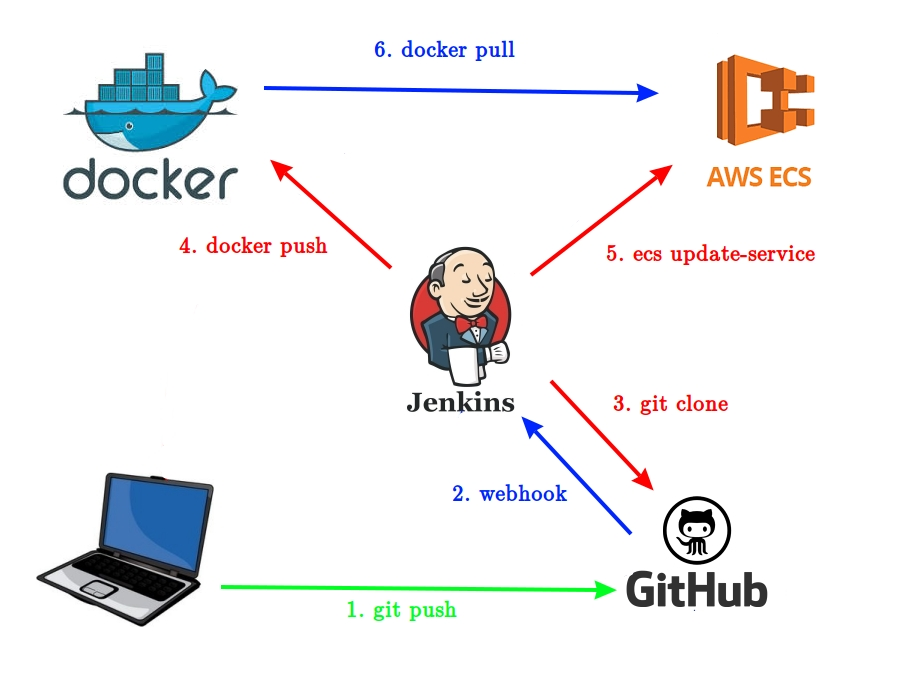
\includegraphics[scale=0.5,keepaspectratio]{cicd}
		\label{fig:cicd}
	\end{figure}
	
	\subsection{JIRA}
	In conjunction with the Scrum framework the Jira development tool will be used. Jira is \deleted[id=RB]{a} a \replaced[id=RB]{project}{porject} management tool which allow the creation and tracking of tasks or issues. The product backlog, comprising of the project user stories, can be created within the management tool with tasks created for each of the stories on the backlog. Each task can then be prioritised as the in the manner chosen by the product owner \citep{jira}.
	
	A number of Jira's feature make it an ideal tool to aid in the organisation of this project:
	\begin{itemize}
		\item \textbf{Issue Tracking:} Progress on issues within the product backlog can be tracked though useful status tags such as In Progress, On Hold and Done. This provides a mechanism for recording progress on each of the user stories which implemented for this project. 
		\item \textbf{Scrum Boards: } Sprints can be represented using Scrum boards. Scrum boards provide a way of organising the issues in a visual manner, grouping them into logical categories (To Do, In Progress, Done) focus on the progress of the current sprint \cite{scruminc}.
	\end{itemize}
	
	\subsection{Completion and Handover}
	Due to the goal driven and iterative aspects of Agile methodology a clear idea of a completed project is required. This will provide a the final goal to work towards and clear understanding of when this goal is reached. Accordingly, a \textit{Definition of Done} is a a key element of Scrum \citep{panchal}. The definition of done for this project shall have the following stipulations:
	\begin{itemize}
		\item All user stories implemented;
		\item All code committed to GitHub repository;
		\item All code documented;
		\item Latest image of web app deployed to ECS through CI/CD;
		\item Latest image available on Docker Hub registry;
		\item A working deployment of the entire system is running and available for demonstration.
	\end{itemize}
	 
	 The following deliverables will be required for completion of the project. 
	 \begin{itemize}
	 	\item Presentation of the project;
	 	\item Project report;
	 	\item Descriptive poster of project;
	 	\item Demonstrative video of project feature.
	 \end{itemize}
     
     \note[id=RB]{This is looking pretty good - you could consider splitting it up into the definition of done for a sprint and the definition of done for the project? Also, check this with Leigh (if you haven't already) to make sure that it meets RedHat's requirements.}